\documentclass{article}
\usepackage{graphicx}
\graphicspath{ {./images/} }
\usepackage{amsmath,amssymb,stackengine}
\usepackage{tikz}
\usepackage{listings}
\usepackage{color}

\definecolor{dkgreen}{rgb}{0,0.6,0}
\definecolor{gray}{rgb}{0.5,0.5,0.5}
\definecolor{mauve}{rgb}{0.58,0,0.82}

\lstset{frame=tb,
	aboveskip=3mm,
	belowskip=3mm,
	showstringspaces=false,
	columns=flexible,
	basicstyle={\small\ttfamily},
	numbers=none,
	numberstyle=\tiny\color{gray},
	keywordstyle=\color{blue},
	commentstyle=\color{dkgreen},
	stringstyle=\color{mauve},
	breaklines=true,
	breakatwhitespace=true,
	tabsize=3
}

\begin{document}
	
	\title{GUI based game: Racket}
	\author{Nikita Melentjevs, Julian Michelsen}
	
	\maketitle
	
	\section{requirements}
	Create a Gui based game using racket, accepting user needs and requirements, 
	visually pleasing functional, bug free final product. \newline
	refining of the problem and posing possible solutions.
	\begin{itemize}
		\item Create a character for the player to control?
		\item Create a level scape for the player to navigate?
		\item Create some way to level up and increase difficulty?
		\item Create enemies of some sort/obstacles?
		\item Create an initial menu screen for the player to choose options and such.
	\end{itemize}
	Possible Solutions:
	\begin{itemize}
		\item portal game
		\item shooter game
		\item geometry dash
	\end{itemize}
	\section{Design}
	Our game is an open-loop system as it relies on the input of the user to create 
	any sort of desired output:
	\begin{itemize}
		\item Our input system is the keyboard where keyboard commands are entered, as well as the cursor and cursor clicks on the initial menu screen.
		\item The controller is the update function, where time is taken into consideration and the user inputs are taken into consideration.
		\item The response is the movement of the player on the GUI.
	\end{itemize}
	\newpage
	\subsection{Top Down Approach}
	Our game is being created with top down design: \\
	where our approach is as follows: \\
	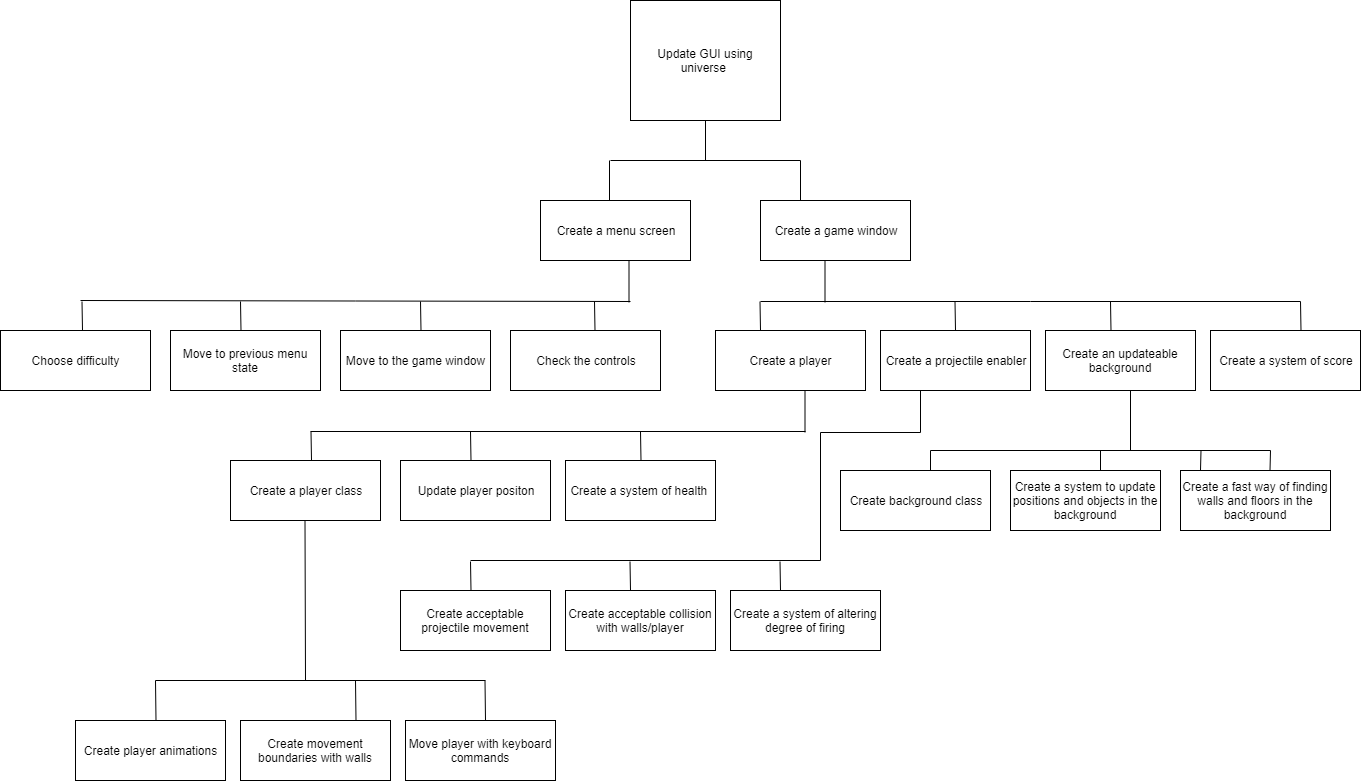
\includegraphics[scale=0.35]{blah1}
	\subsection{Use Cases}
	\begin{itemize}
		\item Create movement through keyboard clicks
		\item Fire a projectile through keyboard clicks
		\item Create a background that looks reasonable
		\item Create enemies to avoid
		\item Create a system of health
		\item Create a system of score
		\item Create animations for the player
		\item Create an acceptable leveling system
	\end{itemize}
	\subsection{UML Class Diagram}
	Write your subsection text here.
	\subsection{Different Data Structures}
	Lists, Hash tables, Sets
	\subsection{FSM's}
	\textbf{Movement through Keyboard Click:} where F represents a check-falling function \\
	Blank line represents time passing.
	\medskip
	\begin{center}
		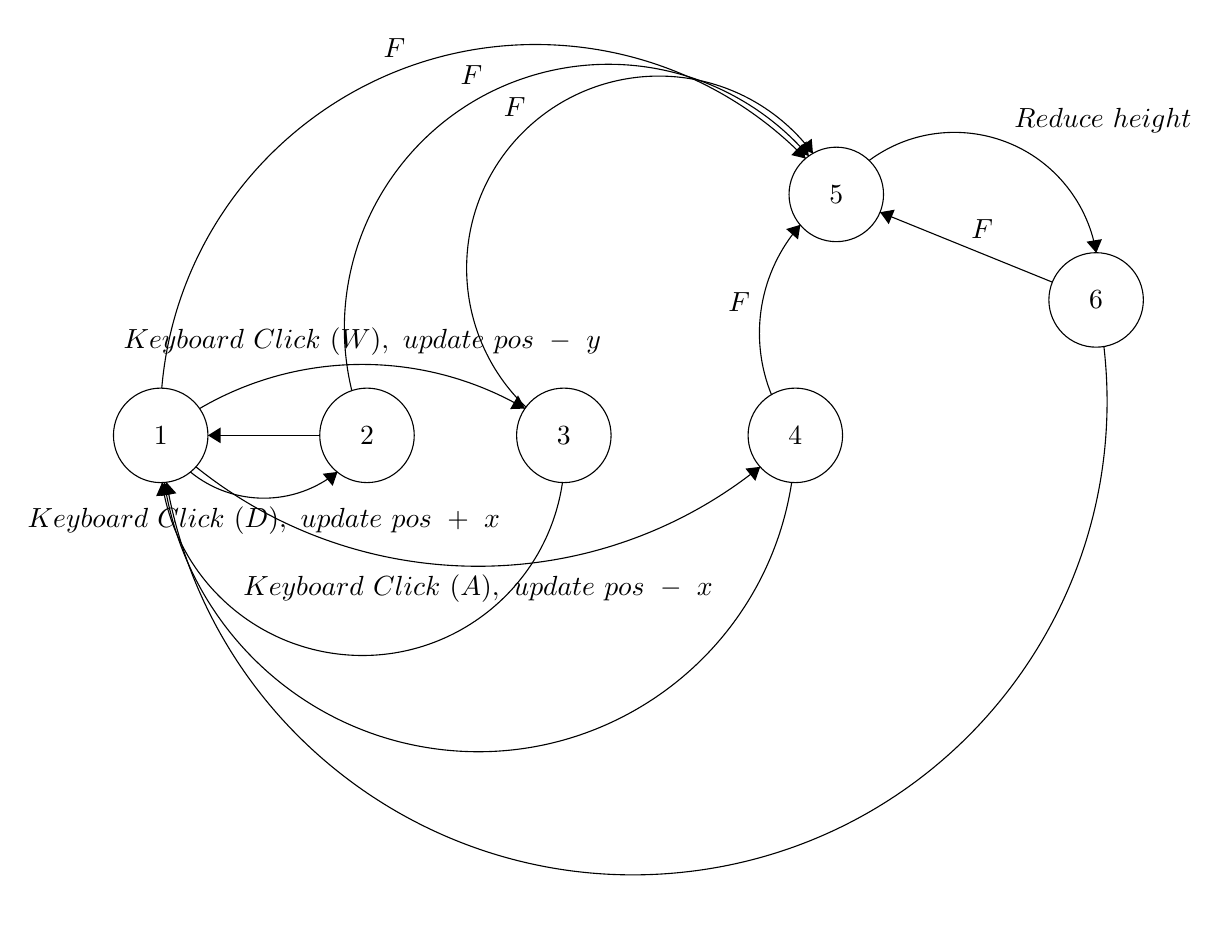
\begin{tikzpicture}[scale=0.2]
		\tikzstyle{every node}+=[inner sep=0pt]
		\draw [black] (8.9,-26.1) circle (3);
		\draw (8.9,-26.1) node {$1$};
		\draw [black] (22,-26.1) circle (3);
		\draw (22,-26.1) node {$2$};
		\draw [black] (34.5,-26.1) circle (3);
		\draw (34.5,-26.1) node {$3$};
		\draw [black] (49.2,-26.1) circle (3);
		\draw (49.2,-26.1) node {$4$};
		\draw [black] (51.8,-10.8) circle (3);
		\draw (51.8,-10.8) node {$5$};
		\draw [black] (68.3,-17.5) circle (3);
		\draw (68.3,-17.5) node {$6$};
		\draw [black] (20.126,-28.416) arc (-50.62992:-129.37008:7.372);
		\fill [black] (20.13,-28.42) -- (19.19,-28.54) -- (19.82,-29.31);
		\draw (15.45,-30.59) node [below] {$Keyboard\mbox{ }Click\mbox{ }(D),\mbox{ }update\mbox{ }pos\mbox{ }+\mbox{ }x$};
		\draw [black] (11.368,-24.399) arc (120.36918:59.63082:20.436);
		\fill [black] (32.03,-24.4) -- (31.59,-23.56) -- (31.09,-24.43);
		\draw (21.7,-21.09) node [above] {$Keyboard\mbox{ }Click\mbox{ }(W),\mbox{ }update\mbox{ }pos\mbox{ }-\mbox{ }y$};
		\draw [black] (46.966,-28.1) arc (-51.17683:-128.82317:28.577);
		\fill [black] (46.97,-28.1) -- (46.03,-28.21) -- (46.66,-28.99);
		\draw (29.05,-34.91) node [below] {$Keyboard\mbox{ }Click\mbox{ }(A),\mbox{ }update\mbox{ }pos\mbox{ }-\mbox{ }x$};
		\draw [black] (8.967,-23.103) arc (-184.8842:-315.85892:23.853);
		\fill [black] (49.85,-8.52) -- (49.65,-7.6) -- (48.94,-8.3);
		\draw (23.75,-2.14) node [above] {$F$};
		\draw [black] (21.037,-23.263) arc (-166.37848:-319.26753:16.777);
		\fill [black] (50.06,-8.36) -- (49.91,-7.43) -- (49.15,-8.08);
		\draw (28.63,-3.88) node [above] {$F$};
		\draw [black] (32.099,-24.313) arc (-133.6994:-323.32196:12.205);
		\fill [black] (50.32,-8.2) -- (50.24,-7.26) -- (49.44,-7.86);
		\draw (31.38,-5.86) node [above] {$F$};
		\draw [black] (47.686,-23.522) arc (-157.85668:-221.43213:10.387);
		\fill [black] (49.52,-12.73) -- (48.62,-13) -- (49.37,-13.66);
		\draw (46.35,-17.63) node [left] {$F$};
		\draw [black] (53.876,-8.653) arc (126.53385:9.26588:9.121);
		\fill [black] (68.31,-14.51) -- (68.67,-13.64) -- (67.69,-13.8);
		\draw (68.73,-6.93) node [above] {$Reduce\mbox{ }height$};
		\draw [black] (65.52,-16.37) -- (54.58,-11.93);
		\fill [black] (54.58,-11.93) -- (55.13,-12.69) -- (55.51,-11.77);
		\draw (61.06,-13.63) node [above] {$F$};
		\draw [black] (68.793,-20.458) arc (6.61329:-170.13708:30.086);
		\fill [black] (9.27,-29.08) -- (8.91,-29.95) -- (9.9,-29.78);
		\draw [black] (48.968,-29.088) arc (-8.70516:-171.29484:20.15);
		\fill [black] (9.13,-29.09) -- (8.76,-29.95) -- (9.75,-29.8);
		\draw [black] (34.414,-29.092) arc (-8.34153:-171.65847:12.85);
		\fill [black] (8.99,-29.09) -- (8.61,-29.96) -- (9.6,-29.81);
		\draw [black] (19,-26.1) -- (11.9,-26.1);
		\fill [black] (11.9,-26.1) -- (12.7,-26.6) -- (12.7,-25.6);
		\end{tikzpicture}
	\end{center}
	\textbf{Code Built from this FSM}
	\begin{lstlisting}
	(cond
	 [(not (equal? 0 animation))
		(if (= direction 0)
			(if (= (send background check-walls (+ x 1) (+ y 16)) 0) 
				(set! x (+ x 1)) #t)
			(if (= (send background check-walls (- x 1) (+ y 16)) 0) 
				(set! x (- x 1)) #t))]
			)]
	(if (and (and (not (equal? animation "jA")) 
			 (not (equal? animation "jD"))) 
		(= (send background check-bases x (+ y 16)) 0))
			(block
			(set! y (+ y 2))
			(set! falling 1) #t)
			(set! falling 0))
	)
	\end{lstlisting}
	\textbf{Portal Relocation:}
	\medskip
	\begin{center}
		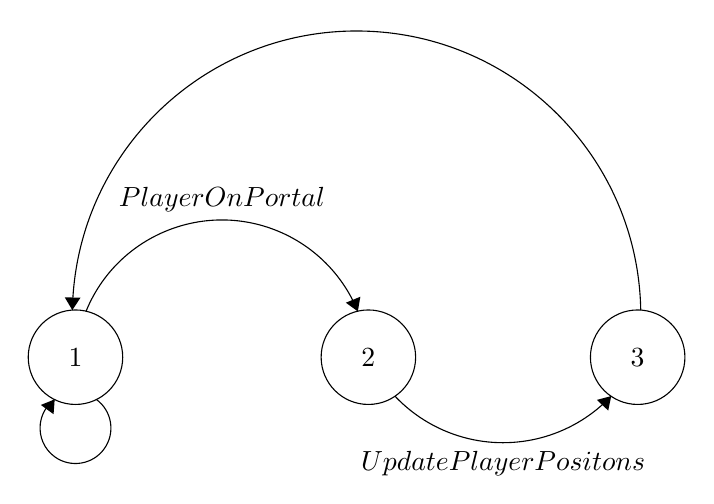
\begin{tikzpicture}[scale=0.2]
		\tikzstyle{every node}+=[inner sep=0pt]
		\draw [black] (11.7,-26.6) circle (3);
		\draw (11.7,-26.6) node {$1$};
		\draw [black] (30.3,-26.6) circle (3);
		\draw (30.3,-26.6) node {$2$};
		\draw [black] (47.4,-26.6) circle (3);
		\draw (47.4,-26.6) node {$3$};
		\draw [black] (12.369,-23.689) arc (157.83031:22.16969:9.32);
		\fill [black] (29.63,-23.69) -- (29.79,-22.76) -- (28.87,-23.14);
		\draw (21,-17.39) node [above] {$PlayerOnPortal$};
		\draw [black] (13.023,-29.28) arc (54:-234:2.25);
		\fill [black] (10.38,-29.28) -- (9.5,-29.63) -- (10.31,-30.22);
		\draw [black] (45.718,-29.069) arc (-43.35936:-136.64064:9.446);
		\fill [black] (45.72,-29.07) -- (44.81,-29.31) -- (45.53,-29.99);
		\draw (38.85,-32.53) node [below] {$UpdatePlayerPositons$};
		\draw [black] (11.505,-23.61) arc (-181.02525:-358.97475:18.048);
		\fill [black] (11.5,-23.61) -- (12.02,-22.82) -- (11.02,-22.8);
		\end{tikzpicture}
	\end{center}
	\medskip
	\textbf{Projectile updating after being fired:}
	\medskip
	\begin{center}
		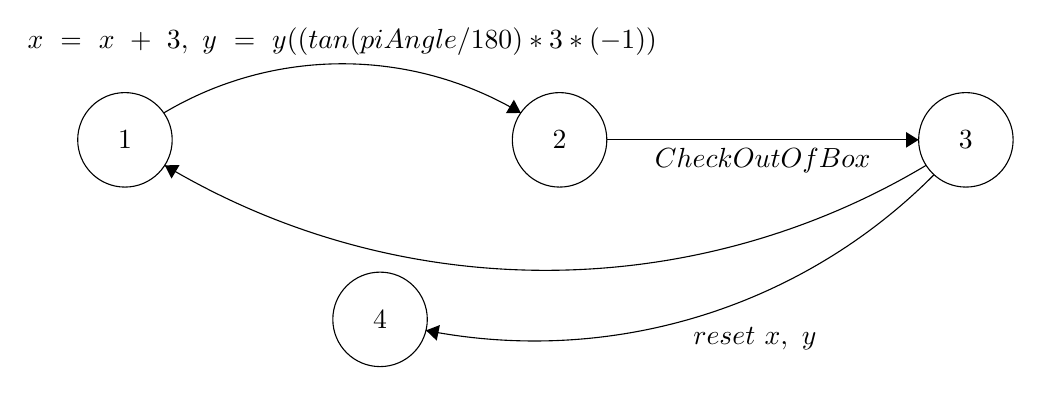
\begin{tikzpicture}[scale=0.2]
		\tikzstyle{every node}+=[inner sep=0pt]
		\draw [black] (9.2,-25.2) circle (3);
		\draw (9.2,-25.2) node {$1$};
		\draw [black] (36.8,-25.2) circle (3);
		\draw (36.8,-25.2) node {$2$};
		\draw [black] (62.6,-25.2) circle (3);
		\draw (62.6,-25.2) node {$3$};
		\draw [black] (25.4,-36.6) circle (3);
		\draw (25.4,-36.6) node {$4$};
		\draw [black] (11.665,-23.493) arc (120.816:59.184:22.127);
		\fill [black] (34.34,-23.49) -- (33.9,-22.65) -- (33.39,-23.51);
		\draw (23,-19.87) node [above] {$x\mbox{ }=\mbox{ }x\mbox{ }+\mbox{ }3,\mbox{ }y\mbox{ }=\mbox{ }y((tan(piAngle/180)*3*(-1))$};
		\draw [black] (39.8,-25.2) -- (59.6,-25.2);
		\fill [black] (59.6,-25.2) -- (58.8,-24.7) -- (58.8,-25.7);
		\draw (49.7,-25.7) node [below] {$CheckOutOfBox$};
		\draw [black] (60.578,-27.415) arc (-44.80789:-101.11658:35.756);
		\fill [black] (28.32,-37.3) -- (29,-37.95) -- (29.2,-36.96);
		\draw (49.2,-37.1) node [below] {$reset\mbox{ }x,\mbox{ }y$};
		\draw [black] (60.075,-26.819) arc (-59.15691:-120.84309:47.153);
		\fill [black] (11.73,-26.82) -- (12.16,-27.66) -- (12.67,-26.8);
		\end{tikzpicture}
	\end{center}
	This FSM was created by reverse engineering the function that we had already created:
	\begin{lstlisting}
	(define (update-projectile angle x y direction)
		(define s1 +)
		(define s2 -)
		(cond
		 [(and (>= angle -90) (<= angle 90)) (set! s2 +)]
		)
		(if (= direction 1) (set! s1 -) #t)
		(set! y (s2 y (* (* (tan (/ (* pi angle) 180)) 3) -1)))
		(set! x (s1 x 3))
		(list x y)
	)
	\end{lstlisting}
	\subsection{EFSM's}
	\textbf{Life reduction EFSM with movement and projectile movement:}
	\begin{center}
		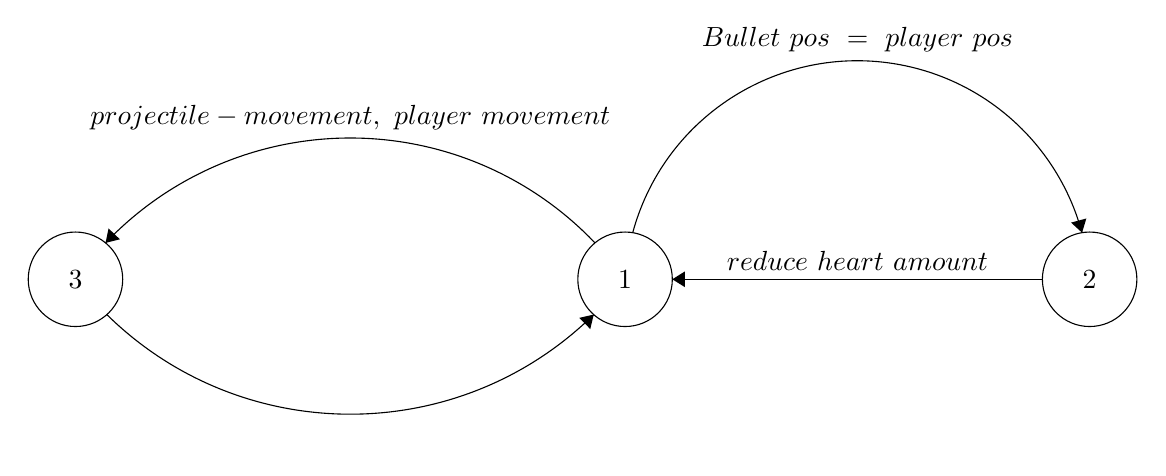
\begin{tikzpicture}[scale=0.2]
		\tikzstyle{every node}+=[inner sep=0pt]
		\draw [black] (42.2,-27.4) circle (3);
		\draw (42.2,-27.4) node {$1$};
		\draw [black] (71.7,-27.4) circle (3);
		\draw (71.7,-27.4) node {$2$};
		\draw [black] (7.3,-27.4) circle (3);
		\draw (7.3,-27.4) node {$3$};
		\draw [black] (42.685,-24.445) arc (164.86988:15.13012:14.778);
		\fill [black] (71.22,-24.44) -- (71.49,-23.54) -- (70.52,-23.8);
		\draw (56.95,-13.02) node [above] {$Bullet\mbox{ }pos\mbox{ }=\mbox{ }player\mbox{ }pos$};
		\draw [black] (9.21,-25.09) arc (136.40934:43.59066:21.456);
		\fill [black] (9.21,-25.09) -- (10.12,-24.86) -- (9.4,-24.17);
		\draw (24.75,-17.93) node [above] {$projectile-movement,\mbox{ }player\mbox{ }movement$};
		\draw [black] (40.21,-29.642) arc (-45.49754:-134.50246:22.056);
		\fill [black] (40.21,-29.64) -- (39.29,-29.85) -- (39.99,-30.56);
		\draw [black] (68.7,-27.4) -- (45.2,-27.4);
		\fill [black] (45.2,-27.4) -- (46,-27.9) -- (46,-26.9);
		\draw (56.95,-26.9) node [above] {$reduce\mbox{ }heart\mbox{ }amount$};
		\end{tikzpicture}
	\end{center}
	\subsection{Human Interface}
	The color background that we have decided to use makes it very easy to distinguish between the walls and the background. The bullet color and the enemy color was chosen to be red as it is the most commonly used color for dangerous objects, so that the player instinctively understands that they should avoid the bullets without being told to. \\ \\
	The star in the interface is also a universal symbol for an object that should be collected. Otherwise player may not know whether or not to move towards it.
	The hearts are placed at the top of the screen to be easily visible by the player.
	\newpage
	\section{Implementation}
	\subsection{Pre-conditions and Post-conditions}
	\textbf{Length Function:}
	\begin{align*}
	&\text{\textbf{Precondition:}} &[x : list \land y = 0] \\
	&\text{\textbf{Postcondition:}} &[y = z \land (x(z) \in x \land x(z + 1) \leftrightarrow \medskip'())] \\
	\end{align*}
	We use : to denote type of a variable. \\ \\
	\textbf{Check Portal Touching Function:} \\
	\begin{align*}
	&\text{\textbf{Precondition:}} &[b-portal \neq \medskip '() \land length(\text{bx b-portal}) \geq 2 \\
	&&\land \medskip length(\text{by b-portal}) \geq 2 \land x \neq \medskip '() \land y \neq \medskip '()] \\ \\
	&\text{\textbf{Postcondition:}} &[y = z \land (x(z) \in x \land x(z + 1) \leftrightarrow \medskip'())]
	\end{align*}
	Where we use (attribute class) to denote class attributes for \\
	specific instantiations of a class
	\subsection{Side Effects}
	The lifebarchange funcion not only changes the amount of hearts the player currently has, but also the bullet class field has-hit, this is an example of where side effects can be very useful, when trigger-checks are updated so that they cannot be triggered again.
	\medskip
	The change function alters almost all the classes in the program, as well as our hash-table that is used for the movement and portal gun rotation. \\
	There are problems that come along with the change function have multiple side effects, such as the difficulty in locating problems in the code and what classes the issue is being created in. \\
	\section{Testing and Maintaining}
	
	\subsection{Test Cases and Assertions}
	\begin{itemize}
		\item {\large \textbf{test cases for player movement}:} \\ \\
			Pressing a while not in air and on platform that is $> 10$ pixels away from
			either a drop or wall to the left of the players character will decrease the players
			x position by $10$ pixels while y stays the same. \\ \\
			$x = x_0 - 10 \land y = y_0$ \\
			
			Pressing d while not in air and on platform that is $>  10$ pixels away from 
			either a drop or wall to the right of the players character will increase the players 
			x position by $10$ pixels while y stays the same. \\ \\
			$x = x_0 + 10 \land y = y_0$ \\
			
			We then gather our test cases and assertions for \textbf{keyboard press a d} \\ \\
			\textbf{Test Cases:}
			\begin{itemize}
				\item \quad player-x = player-x + 10
				\item \quad player-y = player-y
				\item \quad player-x = player-x - 10
			\end{itemize}
			\textbf{Assertions:}
			\begin{lstlisting}
     		(test-begin
			 (cond
				[(and (= (send background check-walls (+ x 10) (+ y 16) 0))
					  (and (not (= (send background check-bases (+ x 10) (+ y 16) 0)))
						   (equal? animation "mD")))
								(check-equal? x (+ x0 10))
								(check-equal? y x0)]
				[(and (= (send background check-walls (- x 10) (+ y 16) 0))
					  (and (not (= (send background check-bases (- x 10) (+ y 16) 0)))
						   (equal? animation "mA")))
								(check-equal? x (- x0 10))
								(check-equal? y x0)]
				)
			)
			\end{lstlisting}
			
		\item {\large \textbf{test cases for teleporting through portals}:} \\ \\
			if the player x position and y position match that of either a blue/orange portal
			then its position is then set to the appropriate x and y position of the other portal. \\ \\
			$blue \to orange$ \\
			$orange \to blue$ \\ \\
			$x = O(x_r + B(x_l - x_0)) \land y = O((y_t - y_b)/2)$  \\ \\
			when going through $B$ portal \\ \\
			$x = B(x_r + O(x_l - x_0)) \land y = B((y_t - y_b)/2)$ \\ \\
			when going through $O$ portal \\ \\
			Here we use $O(y_t)$ and $O(y_b)$ to represent the top and bottom of the y positions of the Orange portal. \\
			we also use $O(x_r)$ and $O(x_l)$ to represent the right and left x values of the Orange portal, we use the same logic for the Blue portal. \\
			
			We then gather our test cases and assertions for \textbf{portal teleporting}. \\ \\
			\textbf{Test Cases:}
			\begin{itemize}
				\item \quad player-x = orange-portal-right-x + player-x - blue-portal-right-x
				\item \quad player-y = orange-portal-top-y - 10
				\item \quad player-y = orange-portal-bottom-y + 10
				\item \quad player-x = orange-portal-right-x + 30
				\item \quad player-y = orange-portal-top-y + player-y - blue-portal-top-y
				\item \quad player-x = orange-portal-right-x - 30
				\item \quad player-y = orange-portal-bottom-y + player-y - blue-portal-top-y
			\end{itemize}
			\textbf{Assertions:}
			\begin{lstlisting}
			(test-begin
			 (cond
				[(equal? (send b-portal get-direction) "d")
					(check-equal? player-x 
								  (+ o-portal-r-x (- player-x0 b-portal-r-x)))
					(check-equal? player-y (- o-portal-y-t 10))]
				[(equal? (send b-portal get-direction) "u")
					(check-equal? player-x
								  (+ o-portal-r-x (- player-x0 b-portal-r-x)))
					(check-equal? player-y (+ o-portal-y-b 10))]
				[(equal? (send b-portal get-direction) "l")
					(check-equal? player-x (+ o-portal-r-x 30))
					(check-equal? player-y 
								  (+ o-portal-t-y 
								  	 (- player-y0 b-portal-t-y)))]
				[(equal? (send b-portal get-direction) "r")
					(check-equal? player-x (- o-portal-r-x 30))
					(check-equal? player-y 
								  (+ o-portal-t-y 
								  	 (- player-y0 b-portal-t-y)))]
				)
			)
			\end{lstlisting}
			And likewise for the blue portal and its assertions and test cases.

		\item {\large \textbf{test cases enemy movement on platforms}:} \\ \\
			When an enemy touches the end of a base platform it moves in the opposite direction \\ \\
			$\iff$ \\ \\
			When there is no platform to $x + (3 * speed)$ of the enemy's x position then it's direction is reversed. \\
			
			we then gather our test cases and assertions for \textbf{enemy movement}. \\ \\
			\textbf{Test Cases:}
			\begin{itemize}
				\item \quad direction = (direction + 1) mod 2
				\item \quad x = x + 1.5*speed
				\item \quad x = x - 1.5*speed
				\item \quad y = y + 2
			\end{itemize}
			\textbf{Assertions:}
			\begin{lstlisting}
			(test-begin
			 (cond
				[(and (and
					(not (= (send background check-bases x (+ y 16)) 0))
					(not (= (send background check-bases (+ x (* 1.5 speed)) (+ y 16)) 0)))
					(= direction 0))
						(check-equal? direction (modulo (+ 1 direction0) 2))
						(check-equal? x (+ x0 (* 1.5 speed)))]
				[(and (and
					(not (= (send background check-bases x (+ y 16)) 0))
					(not (= (send background check-bases (- x (* 1.5 speed)) (+ y 16)) 0)))
					(= direction 1))
						(check-equal? direction (modulo (+ 1 direction0) 2))
						(check-equal? x (- x0 (* 1.5 speed)))]
				[(= (send background check-bases x (+ y 16)) 0)
					(check-equal? y (+ y0 2))
					(check-equal? falling 0)]
				)
			)
			\end{lstlisting}
	\subsection{Specification vs Implementation}
	\end{itemize}
	\subsection{User Feedback}
	survey-link here: https://www.surveymonkey.co.uk/r/FDXDWKN \\ \\
	Data collection and analysis below: \\
	\begin{center}
		\begin{tabular}{ |c|c|c|c| } 
			\hline
			Controls & Look & Enjoyability & Design and Smoothness  \\ 
			\hline
			2.5/5 & 4/5 & 3/5 & 3/5\\ 
			\hline
		\end{tabular}
	\end{center}
	Ratings are an average of all surveys taken / 5 \\ \\
	Amount of surveys taken: 15
	
	\subsection{Amendments from the data}
	\textbf{Controls:} \\ \\
	Controls needed to be improved, we made adjustments to it by
	first adding a section on the menu page labelled controls,
	so that users could understand how the controls worked before actually entering the game,
	we also spaced our the keys that needed to be pressed so that both hands could be used. \\ \\
	\textbf{Look:} \\ \\
	The look of the game was our best part so we decided to focus on other sections which were not as strong. \\ \\
	\textbf{Enjoyability:} \\ \\
	Enjoyability is always a difficult aspect of the game to increase, but by looking at which difficulty users preferred,
	we could gather that the easy mode was the most enjoyable, meaning that we should tweak the other difficulties to be more like the easy mode. Thus we lowered the movement speed of enemies in the 2 other difficulties as well as increasing the time to get the stars. \\ \\
	\textbf{Design and Smoothness:} \\ \\
	To fix issues with lag we implemented binary searches instead of linear searches anywhere we could, this took down the lag by a small margin, but not a noticeable amount.
	
	\subsection{Updated User Feedback}
	\begin{center}
		\begin{tabular}{ |c|c|c|c| } 
			\hline
			Controls & Look & Enjoyability & Design and Smoothness  \\ 
			\hline
			3.5/5 & 4/5 & 3.5/5 & 3.5/5\\ 
			\hline
		\end{tabular}
	\end{center}
	Amount of surveys taken: 12 \\ \\
	As we can clearly see, our adjustments did improve the ratings that we got, but they still were not that high unfortunately.
	
	\section{Conclusion}
	We are happy with our end result, however we would have liked to add some additional features, and reduce the amount of bugs with the portal, however this was taking too much time to complete. Thus we decided to move on with other features of the program. 
	
\end{document}